%%%%%%%%%%%%%%%%%%%%%%%%%%%%%%%%%%%%%%%%%%%%%%%%%%%%%%%%%%%%%%%%%%
%%%%%%%% ICML 2017 EXAMPLE LATEX SUBMISSION FILE %%%%%%%%%%%%%%%%%
%%%%%%%%%%%%%%%%%%%%%%%%%%%%%%%%%%%%%%%%%%%%%%%%%%%%%%%%%%%%%%%%%%

% Use the following line _only_ if you're still using LaTeX 2.09.
%\documentstyle[icml2017,epsf,natbib]{article}
% If you rely on Latex2e packages, like most moden people use this:
\documentclass{article}


\usepackage{csquotes}
% use Times
\usepackage{times}
% For figures
\usepackage{graphicx} % more modern
%\usepackage{epsfig} % less modern
\usepackage{subfigure} 

% For citations
\usepackage{natbib}
\usepackage{booktabs}

% For algorithms
\usepackage{algorithm}
\usepackage{algorithmic}

\usepackage{longtable}
\usepackage{hhline}
\usepackage{booktabs}
\usepackage{array}



\def\specialcell#1{$\vtop{\halign{\hfil##\hfil\strut\cr#1\cr}}$} 

\def\specialcellright#1{$\vtop{\halign{\hfil##\hfil\strut\cr#1\cr}}$}
\newcommand*{\specialcellbold}[2][b]{%
	\bfseries\sffamily
	\begin{tabular}[#1]{@{}c@{}}#2\end{tabular}%
}
 
% As of 2011, we use the hyperref package to produce hyperlinks in the
% resulting PDF.  If this breaks your system, please commend out the
% following usepackage line and replace \usepackage{icml2017} with
% \usepackage[nohyperref]{icml2017} above.
\usepackage{hyperref}

% Packages hyperref and algorithmic misbehave sometimes.  We can fix
% this with the following command.
\newcommand{\theHalgorithm}{\arabic{algorithm}}

% Employ the following version of the ``usepackage'' statement for
% submitting the draft version of the paper for review.  This will set
% the note in the first column to ``Under review.  Do not distribute.''
%\usepackage{icml2017} 

% Employ this version of the ``usepackage'' statement after the paper has
% been accepted, when creating the final version.  This will set the
% note in the first column to ``Proceedings of the...''
\usepackage[accepted]{icml2017}


% The \icmltitle you define below is probably too long as a header.
% Therefore, a short form for the running title is supplied here:
\icmltitlerunning{Machine Learning in Parkinson's Disease Diagnosis.}

\begin{document} 

\twocolumn[
\icmltitle{Feature Engineering and Structured Neural Networks\\ for Parkinson's Disease Diagnosis.}

% It is OKAY to include author information, even for blind
% submissions: the style file will automatically remove it for you
% unless you've provided the [accepted] option to the icml2017
% package.

% list of affiliations. the first argument should be a (short)
% identifier you will use later to specify author affiliations
% Academic affiliations should list Department, University, City, Region, Country
% Industry affiliations should list Company, City, Region, Country

% you can specify symbols, otherwise they are numbered in order
% ideally, you should not use this facility. affiliations will be numbered
% in order of appearance and this is the preferred way.
\icmlsetsymbol{equal}{*}

\begin{icmlauthorlist}
\icmlauthor{Max Wang}{equal,anu}
\end{icmlauthorlist}

\icmlaffiliation{anu}{The Australian National University, Canberra, Australia}

\icmlcorrespondingauthor{Max Wang}{maxwg@outlook.com.au}

% You may provide any keywords that you 
% find helpful for describing your paper; these are used to populate 
% the "keywords" metadata in the PDF but will not be shown in the document
\icmlkeywords{Parkinson's disease diagnosis, machine learning, ICML}

\vskip 0.3in
]

% this must go after the closing bracket ] following \twocolumn[ ...

% This command actually creates the footnote in the first column
% listing the affiliations and the copyright notice.
% The command takes one argument, which is text to display at the start of the footnote.
% The \icmlEqualContribution command is standard text for equal contribution.
% Remove it (just {}) if you do not need this facility.

\printAffiliationsAndNotice{}  % leave blank if no need to mention equal contribution
%\printAffiliationsAndNotice{\icmlEqualContribution} % otherwise use the standard text.

\begin{abstract} 
	No objective test for Parkinson's disease (PD) currently exists, and studies suggest misdiagnosis rates of up to 34 percent. Machine learning presents an opportunity to improve diagnosis; however, the size and nature of datasets makes it difficult to generalise the performance of machine learning models to real world applications. This paper consolidates traditional feature engineering techniques and combines them with deep learning based techniques to develop a strong model for Parkinson's disease diagnosis on a large vocal phonation dataset (mPower). An innovative experimental setup is used to show the potential for machine learning in Parkinson's disease diagnosis.
\end{abstract} 

\section{Introduction}
\label{introduction}
\emph{Parkinson's disease} (PD) will affect around one percent of the population by age 70. It is characterised by the deterioration of dopamine producing neurons in the brain, resulting in symptoms such as abnormal gait, speech, and tremor \cite{savittdiagnosis1}. Current treatments can provide temporary relief from symptoms and slow its progression \cite{slowprog3}; however, cannot repair damage from the disease. Thus, obtaining and accurate early diagnosis is of high importance.

PD is currently diagnosed with a standardised, yet, subjective test administered by a neurologist \cite{tolosadiagnosis26}. PD is not easy to diagnose as only a subset of symptoms are present \cite{thenganatt2014parkinsonsubtypes} and there are many diseases with similar symptoms \cite{parkinsonismdifferential1}. It is especially difficult to diagnose in its early stages, as it is believed that most symptoms manifest once 20-40 percent of dopamine producing neurons have deteriorated \cite{brooksdiagnosis25}. Autopsy is one of the only reliable way to confirm diagnosis, and studies have shown a misdiagnosis rate ranging from 9--34 percent \cite{tolosadiagnosis26, brooksdiagnosis25, jankovic2000evolution}. 

The search for a more objective measure for diagnosis is therefore a ht topic in the research community. Discovering more quantifiable biomarkers such as gene expression \cite{genemarkers} and bodily fluids \cite{biomarkerfluid} is a promising option; however, it is likely that costs will be prohibitive for most early stage patients uncertain about the disease. Machine learning is another viable option, offering an objective and low-cost tool to assist the neurologist in diagnosis.


\section{Machine Learning}
\label{mlpd}
There is major interest in using machine learning to assist in Parkinson's disease diagnosis, and current results are very positive --- often in the high 90s using solely speech or accelerometer data \cite{tsanas2012novel, arora2014high}. However, these results should not be taken at face value --- the experimental setup involves differentiating potentially incorrectly diagnosed PD patients with healthy appearing controls. This simplifies the complexities involved in a neurologist's diagnosis, where they must exclude a number of other causes for the symptoms, and handle early stage patients exhibiting minimal symptoms. 

Furthermore, the datasets associated with these publications often consist of fewer than 40 subjects. Reported results are therefore prone to biases in the dataset and overfitting on cross validation \cite{overfittingcv}. The fact that symptoms such as speech and gait dysfunction are not present in 90 percent of patients suggests that these results occur from some form of overfitting. This is supported by later work consolidating the techniques used in prior work on a new dataset achieving worse results \cite{zhan2016high}.

Considering the issues with current datasets, we would want to ask \textbf{how to evaluate machine learning models}? The obvious option is to create a dataset by monitoring subjects prior to any Parkinsonian symptoms until their passing, where the existence of PD can be confirmed through autopsy. With this longitudinal dataset, we can directly compare the performance of machine learning and neurologists. However, such a dataset would be very costly and logistically difficult to collect --- to advocate for its collection, there needs to be some evidence of machine learning's effectiveness.


The question we are most interested in is:


\begin{displayquote}
	``Can machine learning techniques extract more information than observations from a trained neurologist?''
\end{displayquote}

As neurologist diagnosis relies on judgement from observation, it is possible that some symptoms exhibit in a form imperceptible to a neurologist, but detectable with machine learning on high resolution sensor data. Specifically, we focus on whether speech symptoms imperceptible to the human ear can be detected in microphone data.

A larger dataset is required to ensure that results are statistically significant and not influenced by bias. We chose the mPower dataset, which contains phonations of the vowel /aa/ from 6,000 patients as recorded by an iPhone microphone at 44,100Hz \cite{mpower}. 


\section{Background/Prior Work}
Vowel phonation is an interesting task for diagnosing Parkinson's disease, with evidence that it presents itself earlier than other motor symptoms \cite{earlyvowel}. It avoids many complexities involved in modelling speech and is therefore an easier task in the context of machine learning. Prior works have shown promising results, with \citealt{splittledysphonia2009} and \citealt{tsanas2012novel} obtaining a peak cross validation accuracies of 91.4 and 98.6 percent respectively.

Biologically, speech production consists of two components: the vocal folds and vocal tract. The vocal folds consist of a flap called the \emph{glottis}, which can be opened and closed. During speech production (phonation), air expelled from the lungs causes the glottis to oscillate, producing sound at a range of frequencies. The lowest of these frequencies --- the \textit{fundamental frequency}, \emph{$f_0$} --- correlates to duration of one oscillation and is often denoted the \textit{pitch period}. The vocal tract comprises the components such as the mouth and nose which \textit{shapes} the sound by amplifying and attenuating certain frequencies. The vocal folds and tract can be viewed as a \emph{source-filter model}, where the vocal folds (source) generates the sound (signal) which is shaped by the vocal tract (filter). 

With Parkinson's disease, the impairment of fine motor control reduces control of the glottis, causing incomplete vocal fold closure. The turbulent airflow around the glottis causes a sound described as a `breathy' or `hoarse' voice and results in increased variation over each glottal cycle. This is termed \emph{dysphonia}. A similar phenomenon occurs when the vocal folds are irritated by physical causes such as colds and it is currently unknown whether differentiation between the neurological and physical dysphonia is possible. People with PD also experience hesitant speech from reduction of cognitive ability and slurred or imprecise articulation from 
loss of motor control over the vocal tract. This is termed \emph{dysarthria}.


Although dysarthria is very noticeable to humans, it is more difficult to quantify computationally. Spoken language has a wide variation of accent and styles, and \citealt{hazan2012} shows that models trained on English speakers to not generalize well to German speakers, and vice versa. The Interspeech 2015 competition \cite{compareis15pd} featured a sub-challenge where the extent of PD dysarthria (as rated by the UPDRS) was estimated based on sentence and word pronunciations from 50 patients. The small number of participants greatly limits performance, due to the sheer complexity of modelling speech. \citealt{hahm2015parkinson} used a model to map speech data into \textit{Electromagnetic Articulograph} (EMA) data, representing the movement of the tongue and lips. Features were then extracted on the EMA data to quantify the extent of motor decline. \citealt{orozco2015voiced} showed that the transitions from voiced to unvoiced speech is also a strong indicator of PD.


%\begin{figure}[!htb]
%	\centering\centerline{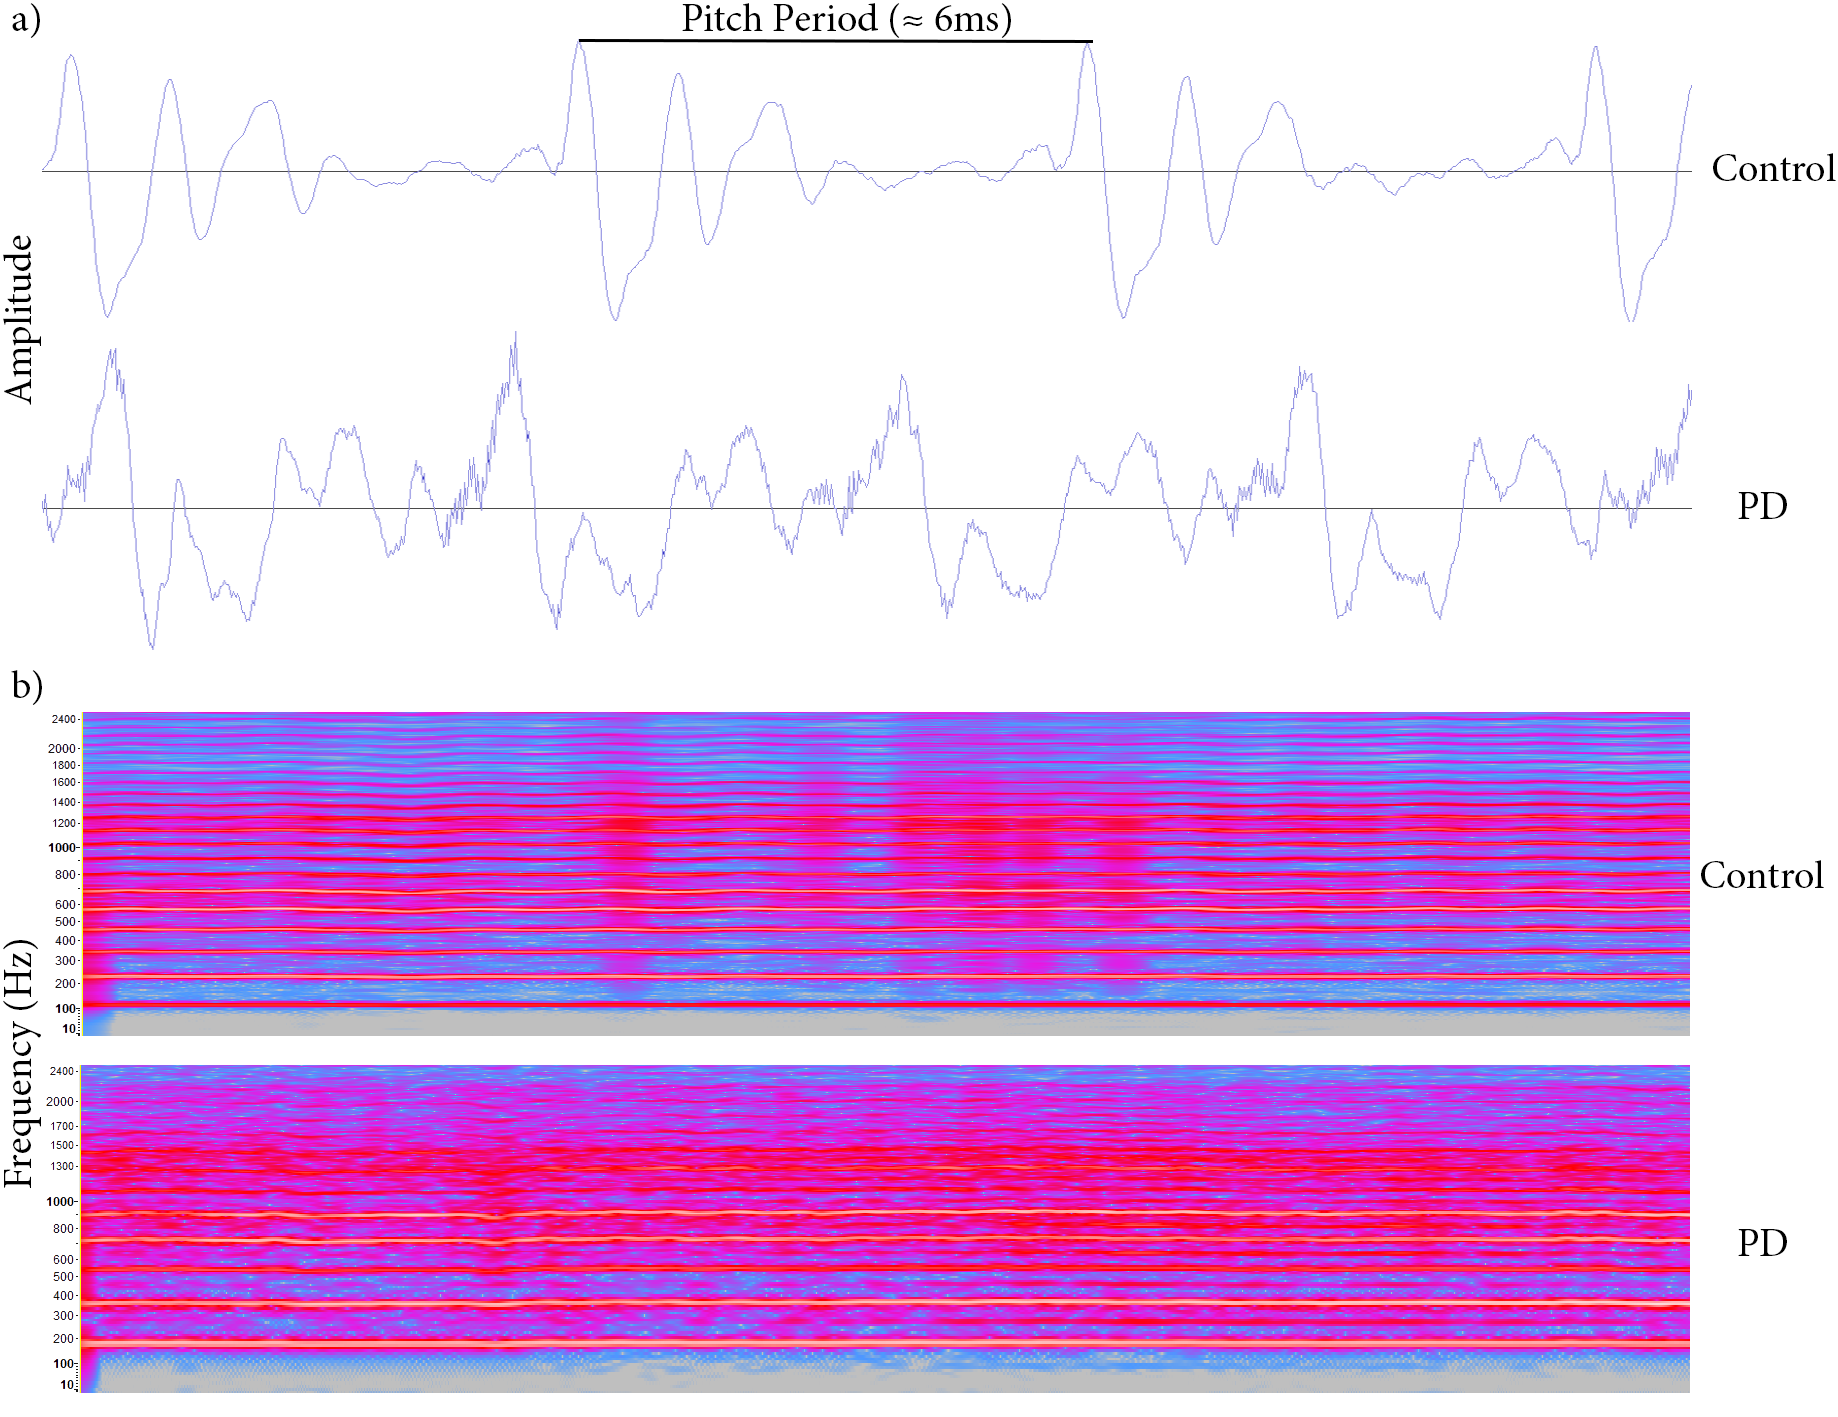
\includegraphics[width=1.2\linewidth]{timespectrogram.png}}
%	\caption{A visualisation of prominent dypshonia in /aa/ phonation on the time (a) and short time spectral domain (b, Mel-scale~\cite{mfscale}). Cases are generally not as extreme and the natural variation in voice makes differentiation a difficult task.}
%	\label{spectrogram}
%\end{figure}


Dysphonia can be measured using \emph{sustained vowel phonations}, which are more suitable for traditional signal processing approaches and small dataset sizes. A visualisation of heavy dysphonia in vowel phonation is presented in \textit{\hyperref[spectrogram]{Figure}} \ref{spectrogram}. Optimally, both dysphonia and dysarthria related features would be used to build models; however, this paper will focus specifically on dysphonia due to availability of data.

\subsection{Features for Dysphonia}
Data from a microphone comes in a stream of numbers, representing the value of the sound wave at each point in time. A basic microphone samples at around 44,100Hz and quantizes the wave to $2^16$ possible values. The difference between higher sampling rates or more detailed quantization (such as 24 bit) is minimally perceptible to human ears --- a bigger issue with low quality microphones is noise and inaccurate sound wave encoding.

Although the raw values can be fed directly into a machine learning model, the assumptions underlying traditional models make them ill equipped to handle the format and size of data. Structured neural networks are the exception.....


Signal processing based approaches calculate features which estimate qualities associated with dysphonia. These features will be divided into three groups: \emph{general} features which are suitable for any time series signal, \emph{dysphonia} specific features, which have been utilised in prior work and \emph{novel} features, which are techniques used for other applications which we believe to be effective in quantifying dysphonia.

 
\subsubsection{General Signal Processing}
\emph{Moments} are basic statistical descriptors of a signal, with the first three moments representing mean, variance, skewness. For speech, mean is largely uninformative and variance corresponds to volume. The \emph{zero crossing rate} measures how quickly the signal oscillates around zero and is a measure of signal frequency. \emph{Entropy} describes the amount of information in a piece of data, if it were modelled by a Bernoulli scheme. It is a simple measure of the complexity/detail in a signal. 


The \emph{Fourier} transform decomposes a signal into the amplitudes of frequencies that compose it. This is referred to as mapping from the \textit{time} domain to the \textit{frequency}, or \textit{spectral} domain. For speech, this enables us to determine the frequency bands with more energy --- corresponding to the the fundamental frequency and harmonics. After performing a Fourier transform, the \emph{spectral entropy} can be calculated, which can measure how `sharp' the $f_0$ and harmonics of speech is. People with PD are expected to have a lower spectral entropy due to the less precise frequency control causing a more `blurred' Fourier transform.

Energy operators such as the Squared (\emph{SEO}) or Teager-Kaiser (\emph{TKEO}) \cite{tkeo} can obtain the instantaneous frequency and amplitude of a signal. Statistics such as mean or standard deviation, and other measures can be computed after the result of applying an energy operator.

\subsubsection{Dysphonia Signal Processing}
From figure XXX, the major features present in dysphonic speech is the increased variation between each glottal cycle. \emph{Jitter}~ measures the variation in the length of each glottal cycle, and \emph{shimmer}~\cite{shimmerjitter} the variation in amplitude. These often rely on detecting each glottal cycle --- which is not very accurate with current algorithms~\cite{f0estimation}. The harmonics-to-noise ratio (\emph{HNR}~\citealt{HNRintro}) measures the amount of noise in a signal, which correlates with the `hoarseness' or `breathiness' of speech. The HNR was improved with the more robust Glottal to Noise Excitiation ratio (\emph{GNE}, \citealt{gne}).


The Vocal Fold Excitation Ratio (\emph{VFER}) is another extension of the HNR developed by \citealt{tsanas2011nonlinear}; who also introduces the Glottal Quotient (\emph{GQ}), a measure of the duration the glottis is opened versus closed. Both VFER and GQ are built upon concepts of the DYPSA~\cite{dypsa} fundamental frequency estimation algorithm. 

Mel-Frequency Cepstral Coefficients (\emph{MFCC}) have long been used for speech recognition~\cite{mfcc}, and also show promise in detecting dysphonia~\cite{mfccml}. They are the most common and often the only feature used in speech recognition systems, but they lack interpretability and are very sensitive to noise~\cite{mfccrobust}. There are also a variety of feature sets used in general speech classification, such as the 6,368 feature ComParE set~\cite{is2013}. Although these features may not be designed specifically for dysphonia, they are effective in fields such as speaker trait classification and may be useful in providing contextual information for complex machine learning models. The incidence of PD varies based on age, gender and race~\cite{ageracial,racial}, and it is likely that dysphonia presents itself differently depending on speaker traits. We refer to Eyben~\cite{ostextbook} for a comprehensive description of these features as well as a summary of feature sets used in speech classification.


\label{dfadescription}
Methods used in non-linear dynamical systems\footnote{Dynamical systems theory is used to describe the behaviour of deterministic systems which appear to exhibit unpredictable behaviour based on a number of initial conditions. This will be explored further in \textit{\hyperref[eegsigproc]{Section}} \ref{eegsigproc}} have also been effective in dysphonia quantification~\cite{splittlenonlinear2007}. \textit{Detrended Fluctuation Analysis} (\emph{DFA}) was originally introduced as a measure of the autocorrelation\footnote{\emph{Autocorrelation} describes the similarity of a signal to itself when offset by a given interval.} of a signal~\cite{dfa}. Little~et~al.~\cite{splittlenonlinear2007} shows this correlates with the amount of turbulent airflow in speakers with dysphonia. Little~et~al. also proposes Recurrence Period Density Entropy (\emph{RPDE}), which characterises the periodicity of a signal. These measures are expected to be lower for speakers with dysphonia due to the noise introduced by turbulent airflow. Little~et~al.~\cite{splittledysphonia2009} builds upon RPDE to develop Pitch Period Entropy (\emph{PPE}) which is a better measure of the impaired control of pitch experienced by PD patients.


%\begin{longtable}{r p{114mm}}
%	\caption{Dysphonia signal processing generally quantifies the variation in each glottal cycle during speech production}\\
%	\multicolumn{2}{c}{\specialcellbold{Voice -- Dysphonia}} \\
%	\midrule
%	\specialcellright{Power\\Cepstrum} & From the inverse Fourier transform. Commonly taken in the Mel-log scale~\cite{mfscale}, resulting in the MFCC~\cite{mfcc}. Minimal interpretability, though it is the primary feature used in speech recognition~\cite{mfccml}. \\
%	Pitch~\cite{f0estimation} & Although obtainable with a Fourier transform, pitch often refers to estimating the exact duration of each glottal cycle.\\
%	Loudness & The volume of a sound in relation to human hearing. Only meaningful if recording setup is strictly controlled.\\
%	Formants & The resonance frequencies of an audio sample.\\
%	HNR~\cite{HNRintro,HNRperiodic} & Measures the ratio of noise in a voiced signal (signal to noise)\\
%	Jitter~\cite{jittertime} & Measures of the variation between the length of each glottal cycle. \\
%	Shimmer~\cite{shimmerjitter} & Measures of the variation of amplitude between each glottal cycle. \\
%	LPCC~\cite{lpcc} & Coefficients of an \textit{autoregressive} model which measures how well a signal can be modelled linearly by its previous values.\\
%	GNE~\cite{gne} & An extension of HNR by Michaelis et~al.~\cite{gne} to improve reliability in dysphonia quantification. \\
%	VFER~\cite{tsanas2012novel} & An further extension of HNR, building upon the theory of GNE.\\
%	EMD-ER~\cite{EMDER} & Another technique developed based on non-linear speech theory to quantify signal to noise\\
%	GQ~\cite{tsanas2012novel} & Measures standard deviation of duration the glottis is opened vs. closed.\\
%	DFA~\cite{splittlenonlinear2007, dfa} & Detrended Fluctuation Analysis. A generalisation of the Hurst exponent which measures the autocorrelation of a time series.\\
%	RPDE~\cite{splittlenonlinear2007} & Measures the periodicity of a signal, specifically designed with non-linear speech as the target.\\
%	PPE~\cite{splittledysphonia2009} & Measures the stability of pitch in sustained phonation.	\\
%	\specialcellright{\hspace{1.9em}Wavelet\\Measures~\cite{sptsanastelemonitor2010}} & A set of 180 measures for dysphonia based on wavelet transforms to the $f_0$ of speech introduced by Tsanas~et~al.~\cite{tsanas2011nonlinear}.\\
%	\specialcellright{GeMAPS~\cite{geneva}} & A minimal acoustic feature set of 58 or 87 (eGeMAPS) parameters that performs well in general speech classification~\cite{ostextbook}.\\
%	\specialcellright{\hspace{1.3em}Interspeech\\ComParE~\cite{compareis13featureset}} & An exhaustive 6,368 feature set for general speech classification~\cite{ostextbook}. Feature/dimensionality reduction generally improves performance unless data is plentiful.
%	%\\\specialcellright{Hammarberg\\ \hspace{0.2em} Index~\cite{hammarberg1980perceptual}} & The ratio of the strongest energy peak from 0-2kHz versus 2-5kHz. The \textit{Alpha Ratio} is similar, measuring the largest peak 50Hz-1kHz versus 1kHz-5kHz.\\
%	\\
%	\midrule
%\end{longtable}
%
%
%\begin{longtable}{r p{114mm}}
%	\caption{There are few movement specific features, with most based on simple measures of postural sway or irregular gait.}\\
%	\multicolumn{2}{c}{\specialcellbold{Movement}} \\
%	\midrule
%	\specialcellright{\hspace{2.5em}Fourier\\\hspace{2.7em}Bands} & The power in bands such as 3.5hz-7hz compared to 7hz-12hz are the primary features used to detect Parkinsonian tremor.\\
%	Jerk~\cite{jerkfeature} & The change in acceleration. The jerk signal may be more effective when combined with certain signal processing methods.\\
%	\specialcellright{Sway\\Area} & This can be calculated na\"{i}vely by multiplying the range of sway in the A/P and M/L directions or by fitting a bounding ellipse in the principal component axis~\cite{pcasway}. As A/P and M/L directions are lost in accelerometer data, the bounding ellipse method is used.\\
%	\specialcellright{Cadence\\Measures} & The steps per minute, variation in time taken for each step, difference between left and right stride times.\\
%	\specialcellright{\hspace{1em}Stride\\Measures} & The length of each step and variation in step lengths. This was not measured as leg length is not available in the dataset used~\cite{diaz2014step}.
%	\\ 
%	\midrule
%\end{longtable}
%
%\vspace{2em}
%
%\begin{longtable}{r p{114mm}}
%	\caption{EEG signal processing is often based on non-linear systems theory. These features may be effective in detecting the presence of symptoms invisible to neurologists.}
%	\label{eegfeatsum}\\
%	\multicolumn{2}{c}{\specialcellbold{EEG}} \\
%	\midrule
%	\specialcellright{\hspace{3.6em}Hjorth\\Parameters~\cite{hjorth}} & Three simple statistical measurements of a signal which have been used as features in EEG and IMU models~\cite{hjorthsmartphone}.\\
%	\specialcellright{\hspace{2em}Lyapunov\\Exponents~\cite{eckmann1986liapunov}} & Characterises the divergence of systems with close initial conditions. The largest exponent ($\lambda^*$)~\cite{dingwell2000nonlinearlyapunov} is generally the most informative. \\
%	\specialcellright{\hspace{3.3em}Fractal\\Dimension~\cite{mandelbrot1967long}} & A measure of how the detail in a signal changes with the scale at which it is measured. The Higuchi~\cite{hfd} and Petrosian~\cite{petrosian1995kolmogorov} fractal dimensions are used in this thesis.\\
%	\specialcellright{\hspace{3.2em}Hurst\\Exponent~\cite{hurst}} & Characterises self-similarity. DFA is a generalisation of the Hurst Exponent and is robust to non-stationary signals. The difference in measurements may be informative.\\
%	\specialcellright{Fisher Info~\cite{fisherinfo2}} & Quantifies the non-linear dynamics in the system generating a signal.\\
%	\specialcellright{\hspace{1.1em}Ap/Samp\\Entropy~\cite{apentropy}} & Approximate and sample entropy quantify the unpredictability of a signal. Multiscale entropy increases information content~\cite{multiscaleentropy}.\\
%	\specialcellright{Spectral\\Entropy} & Measures the regularity of the spectral (frequency) distribution. A high spectral entropy implies sharp differences in frequencies present in the signal.\\
%	\specialcellright{\hspace{2.9em}SVD\\Entropy~\cite{svdentropy}} & A measure of complexity. The entropy of the singular values of the signal after applying the time delay embedding method~\cite{rosenstein1993practicallyapunov}.
%	\\
%	\midrule
%\end{longtable}
%
%
%Early dysphonia analysis is based on variations of jitter, shimmer, and the harmonics-to-noise ratio. \emph{Jitter}~ measures the variation in the length of each glottal cycle, and \emph{shimmer}~\cite{shimmerjitter,jittertime} the variation in amplitude (volume). The harmonics-to-noise ratio (\emph{HNR})~\cite{HNRintro} measures the amount of noise in a signal, which correlates with the `hoarseness' or `breathiness'of speech, which arises from the incomplete closure of the glottis.  The Glottal to Noise Excitation (\emph{GNE}) ratio was introduced by Michaelis~et.al~\cite{gne} and is a more robust measure of dysphonia than HNR~\cite{gneratio}. 


TODO:: DISCUSS CURSE OF DIMENSIONALITY


\section{Our Work}
A major issue with the mPower dataset is the dataset quality --- as it is crowd-sourced, there is significant noise from



\bibliography{icml}
\bibliographystyle{icml2017}

\end{document} 

